% Yampa-IY.tex
\begin{hcarentry}[updated]{Yampa}
\report{Ivan Perez}%11/17
\label{yampa}
\makeheader

Yampa (Github: \href{http://git.io/vTvxQ}{http://git.io/vTvxQ}, Hackage:
\href{http://goo.gl/JGwycF}{http://goo.gl/JGwycF}), is a Functional Reactive
Programming implementation in the form of a EDSL to define \emph{Signal
Functions}, that is, transformations of input signals into output signals (aka.
\emph{behaviours} in other FRP dialects).

Yampa systems are defined as combinations of Signal Functions.  Yampa includes
combinators to create constant signals, apply  pointwise (or time-wise)
transformations, access the running time, introduce delays and create loopbacks
(carrying present output as future input). Systems can be dynamic: their
structure can be changed using \emph{switching} combinators, which apply a
different signal function at some point in the future. Combinators that deal
with collections enable adding, removing, altering, pausing and unpausing
signal functions at will.

A suitable thinking model for FRP in Yampa is that of signal processing, in
which components (signal functions) transform signals based on their present
value and a component's internal state. Components can, therefore, be
serialized, applied in parallel, etc. Yampa's signal functions implement the
Arrow and ArrowLoop typeclasses, making it possible to use both arrow
notation and arrow combinators.

Yampa combinators guarantee \emph{causality}: the value of an output signal at
a time $t$ can only depend on values of input signals at times $[0,t]$.
Efficiency is provided by limiting history only to the immediate past, and
letting signals functions explicitly carry \emph{state} for the future.  Unlike
other implementations of FRP, Yampa enforces a strict separation of effects and
pure transformations: all IO code must exist outside Signal Functions,
making systems easier to reason about and debug.

Yampa has been used to create both free/open-source and commercial games.
Examples of the former include Frag (\href{http://goo.gl/8bfSmz}{http://goo.gl/8bfSmz}), a basic
reimplementation of the Quake III Arena engine in Haskell, and Haskanoid
(\href{http://git.io/v8eq3}{http://git.io/v8eq3}), an arkanoid game featuring
SDL graphics and sound with Wiimote \& Kinect support, which works on Windows,
Linux, Mac, Android and web browsers (thanks to GHCJS). Examples of the latter
include Keera Studios' Magic Cookies!
(\href{https://goo.gl/0A8z6i}{https://goo.gl/0A8z6i}), a board game for Android
written in Haskell and avaliable on Google Play.

%**<img width=700 src="./androidbreakout.png">
%*ignore
\begin{center}
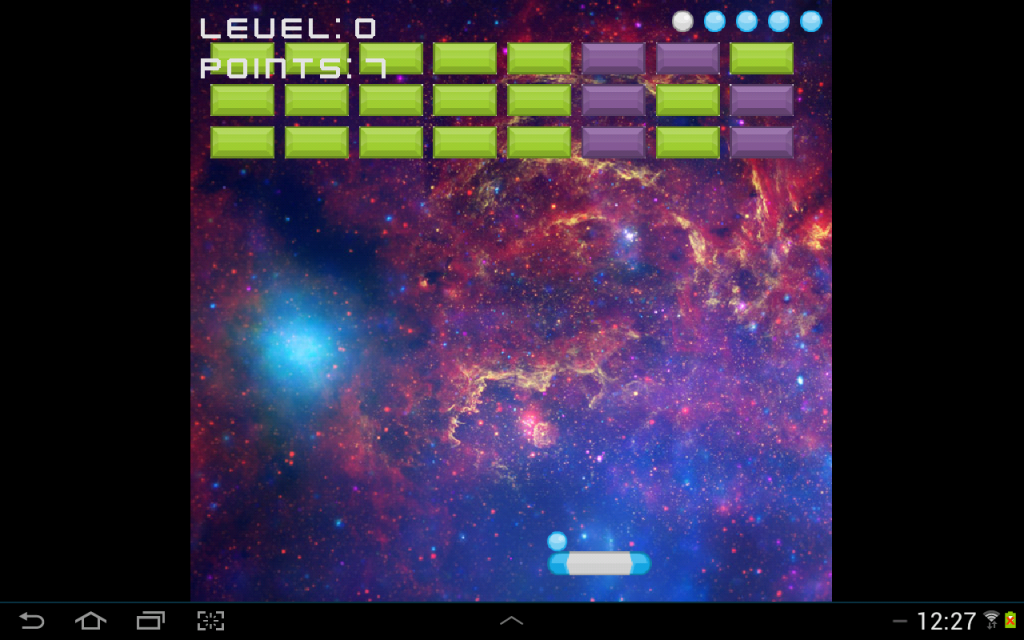
\includegraphics[width=.7\columnwidth]{html/androidbreakout.png}
% \caption{Screenshot of Yampa game Haskanoid running on Android.}
\end{center}
%*endignore

Guerric Chupin (ENSTA ParisTech), under the supervision of Henrik Nilsson
(Functional Programming Lab, University of Nottingham) has developed Arpeggigon
(\href{https://gitlab.com/chupin/arpeggigon}{https://gitlab.com/chupin/arpeggigon}),
an interactive cellular automaton for composing groove-based music. The aim was
to evaluate two reactive but complementary frameworks for implementing
interactive time-aware applications. Arpeggigon uses Yampa for music
generation, Gtk2HS for Graphical User Interface, jack for handling MIDI I/O,
and Keera Hails to implement a declarative MVC architecture, based on
\emph{Reactive Values and Relations} (RVRs).  The results have been written up
in an application paper, \emph{Funky Grooves: Declarative Programming of
Full-Fledged Musical Applications}, presented at PADL 2017. The code and an
extended version of the paper are publicly available
(\href{https://gitlab.com/chupin/arpeggigon}{https://gitlab.com/chupin/arpeggigon}).
Arpeggigon has also been demonstrated at FARM 2017, the Haskell eXchange 2017,
and Haskell in Leipzig 2017. 

%**<img width=700 src="./arpeggigon.png">
%*ignore
\begin{center}
  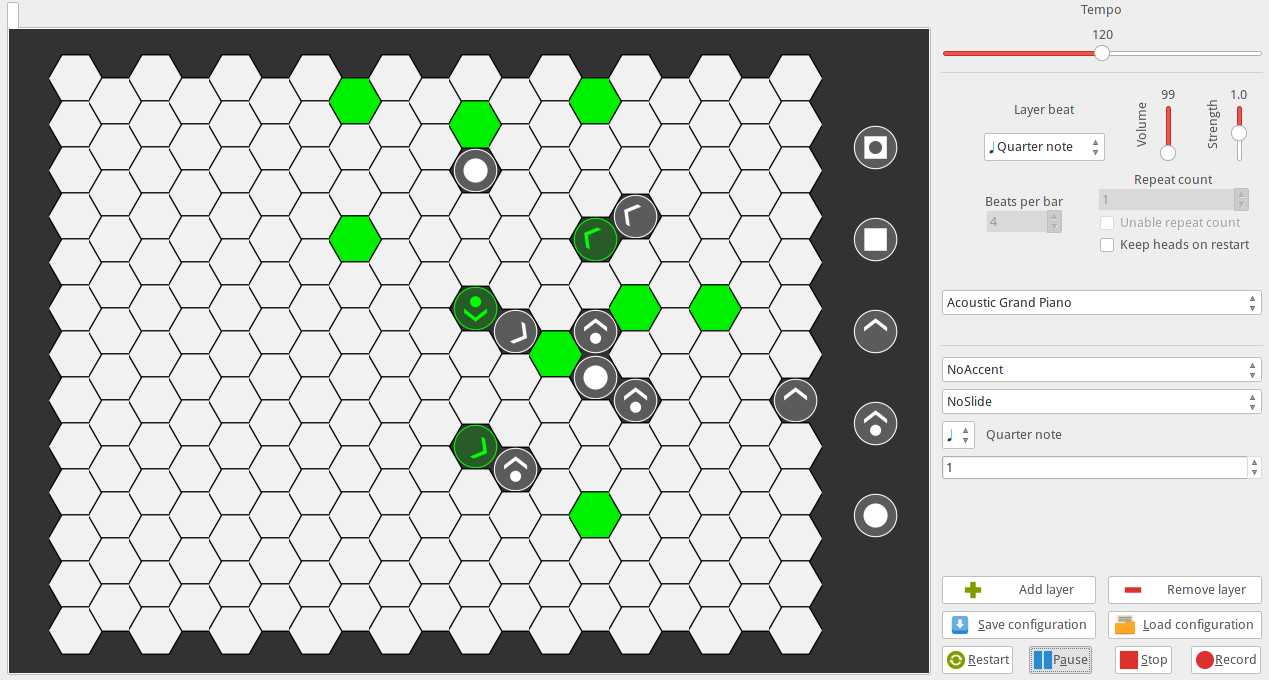
\includegraphics[width=.7\columnwidth]{html/arpeggigon.png}
  % \caption{Screenshot of Guerric Chupin's Arpeggigon, which combines Reactive Values
  % and FRP.}
\end{center}
%*endignore

Yampa is under active development, with many Haskellers  participating on
github and sending their contributions. The last few versions of Yampa have
featured a cleaner API, better documentation and new Signal Function
combinators. Our github repository includes development branches with features
that have been used to extend Yampa for custom games. Some of these features
have been presented in the paper ``Back to the Future: time travel in FRP'',
presented at the Haskell Symposium 2017, and will be included in future
versions. Yampa will now be extended with testing and debugging features, which
allow us to express temporal assertions about FRP systems using Temporal Logic,
and to use QuickCheck to test those properties, as described in the paper
``Testing and Debugging Functional Reactive Programming'', presented at ICFP
2017. 

Extensions to Arrowized Functional Reactive Programming are an active research
topic. Last year we published, together with Manuel B\"arenz, a monadic
arrowized reactive framework called Dunai
(\href{https://git.io/vXsw1}{https://git.io/vXsw1}), and a minimal FRP
implementation called BearRiver. BearRiver provides all the core features of
Yampa, as well as additional extensions. We have demonstrated the usefulness of
our approach and the compatibility with existing Yampa games by using BearRiver
to compile and execute the Haskanoid and Magic Cookies! for Android without
changing the code of such games. These games are also available for iOS and
other platforms.

The Functional Programming Laboratory at the University of Nottingham is
working on other extensions to make Yampa more general and modular, increase
performance, enable new use cases and address existing limitations. To
collaborate with our research, please contact Ivan Perez
(\href{mailto:ixp@cs.nott.ac.uk}{ixp@cs.nott.ac.uk}) and Henrik Nilsson
(\href{mailto:nhn@cs.nott.ac.uk}{nhn@cs.nott.ac.uk}).

We encourage all Haskellers to participate on Yampa's development by opening
issues on our Github page (\href{http://git.io/vTvxQ}{http://git.io/vTvxQ}),
adding improvements, creating tutorials and examples, and using Yampa in their
next amazing Haskell games. We thank the kind users who have already sent us
their pull requests.
\end{hcarentry}
